\chapter{Results}

The data from a total of 23 participants with the average of 335 and a total of 7708 trials were used for the analysis. The starting location IDs were identical with the building-IDs inside the unity environment and were not replaced with new numbers for the analysis.

\section{Summary statistics of dependent variables}

\subsection{Absolute angular deviation}

This variable has the mean of 48.08 with the standard deviation of 44.30, and median of 33.70. (See figure \ref{fig:angular_dev_dists})

\begin{figure}[h]
	\centering
	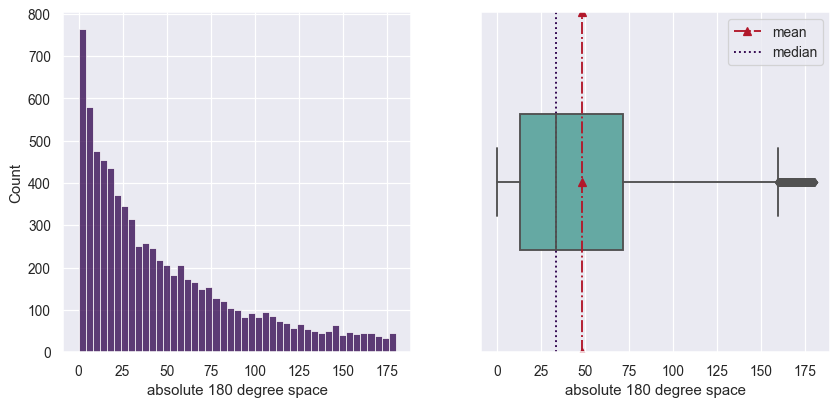
\includegraphics[width=150mm]{figures/angular_deviation_hist_box_23.png}
	\caption[Distribution of the absolute angular deviation]{distribution of the absolute angular deviation}
	\label{fig:angular_dev_dists}
\end{figure}

\subsection{Reaction times}

This variable has the mean of 7.77 with the standard deviation of 5.56, and median of 6.06. (See figure \ref{fig:rt_dists})

\begin{figure}[h]
	\centering
	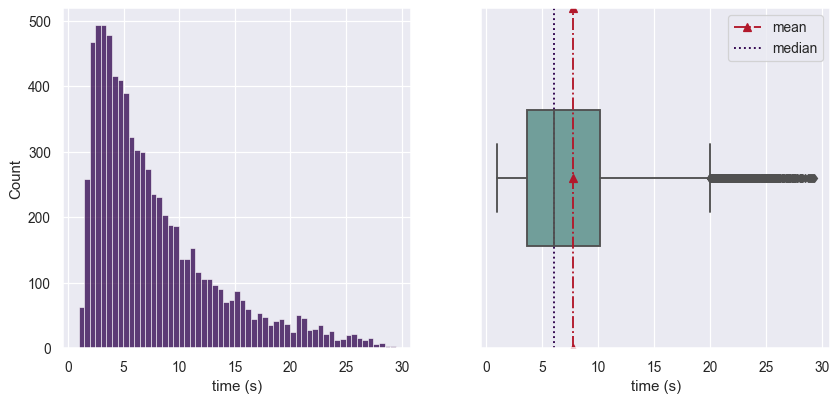
\includegraphics[width=150mm]{figures/RT_hist_box_23.png}
	\caption[Distribution of reaction times]{distribution of the  reaction times in the pointing task}
	\label{fig:rt_dists}
\end{figure}

\section{Extremes at starting locations}

\subsection{Absolute angular deviation}

In order to find out which of the 28 starting locations were the best and worst in performance with respect to the angular deviation from the target, the minimum and maximum medians of angular deviation grouped by the starting locations were taken.\\
As a result the starting location with the ID 9 which is a "patisserie" shop, therefore a context meaningful location, with the median of 19.18 degree deviation from the targets and the difference of 16.03 degree from the overall median (35.21) is the best location, i.e., has the lowest degree deviation from the target. See figure \ref{fig:best_angular}.\\

\begin{figure}[h!]
	\centering
	\begin{subfigure}[b]{0.48\linewidth}
		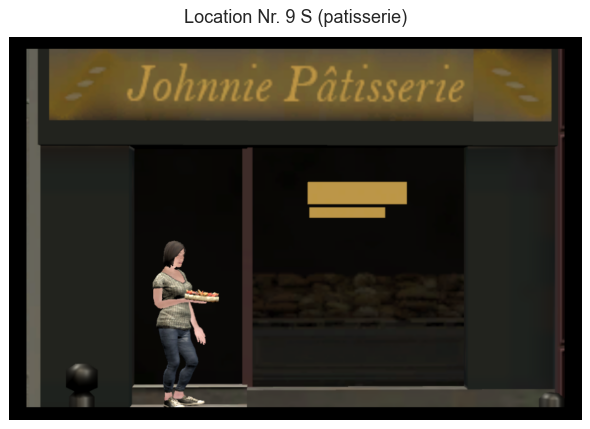
\includegraphics[width=\linewidth]{figures/best_loc_angular_error_withHA_23.png}
		\caption{best starting location}
		\label{fig:best_angular}
	\end{subfigure}
	\begin{subfigure}[b]{0.48\linewidth}
		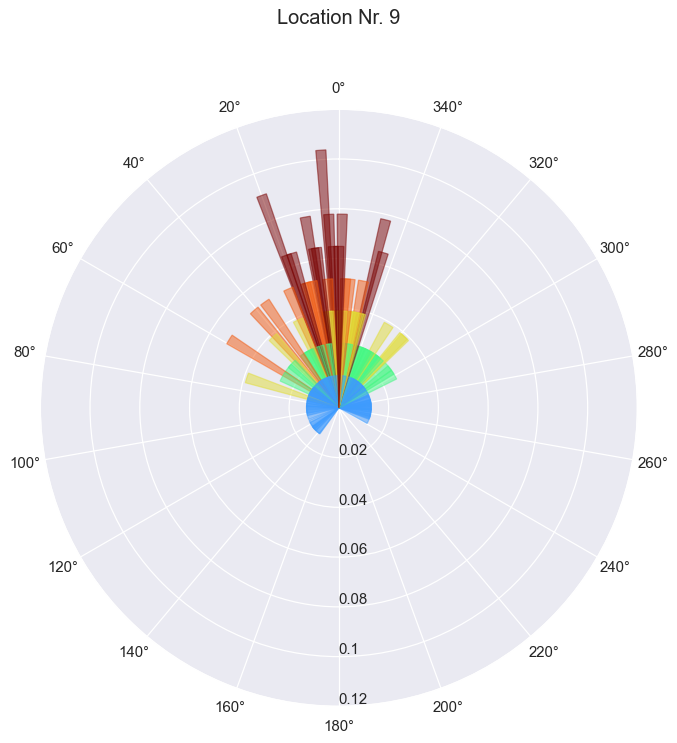
\includegraphics[width=\linewidth]{figures/deviation_degrees_loc_nr_9_23.png}
		\caption{angular deviation in location 9 (\%)}
		\label{fig:best_angular_dist_9}
	\end{subfigure}
	
	\caption[Best starting location based on angular deviation]{the best starting location is chosen by taking the least median angular deviation among all starting locations.}
\end{figure}
\label{fig:best_location}

Furthermore, the starting location with the ID 35, one of the residential, thus not context meaningful, buildings with the angular deviation median of 52.49 degree away from the target and overall distance of 17.28 degree from the overall median (35.21) was the worst location of performing the task with regard to the angular deviation. See figure \ref{fig:worst_angular}.

\begin{figure}[!h]
	\begin{subfigure}[b]{0.48\linewidth}
		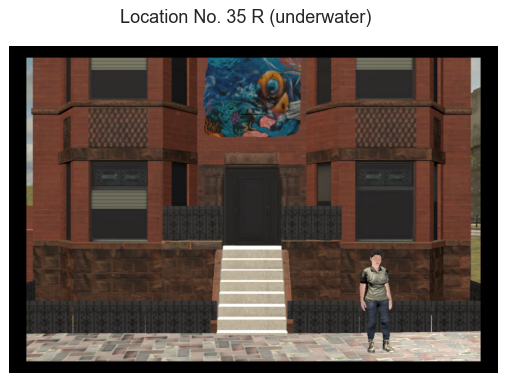
\includegraphics[width=\linewidth]{figures/worst_loc_angular_error__withHA_23.png}
		\caption{worst starting location}
		\label{fig:worst_angular}
	\end{subfigure}
	\begin{subfigure}[b]{0.48\linewidth}
		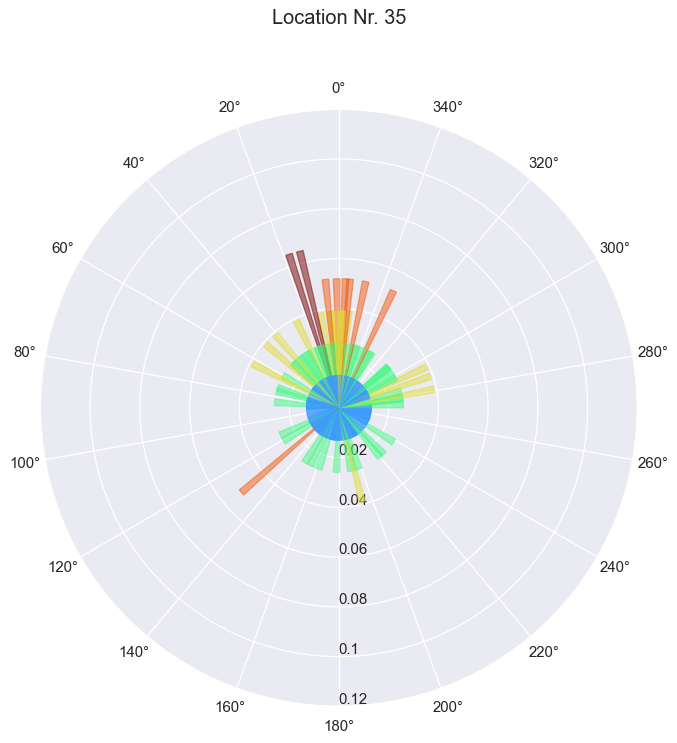
\includegraphics[width=\linewidth]{figures/deviation_degrees_loc_nr_35_23.png}
		\caption{angular deviation in location 35 (\%)}
		\label{fig:worst_angular_dist_35}
	\end{subfigure}

	\caption[Worst starting location based on angular deviation]{the worst starting location is chosen by taking the highest median angular deviation among all starting locations.}
\end{figure}
\label{fig:worst_location}

\begin{figure}[h]
	\centering
	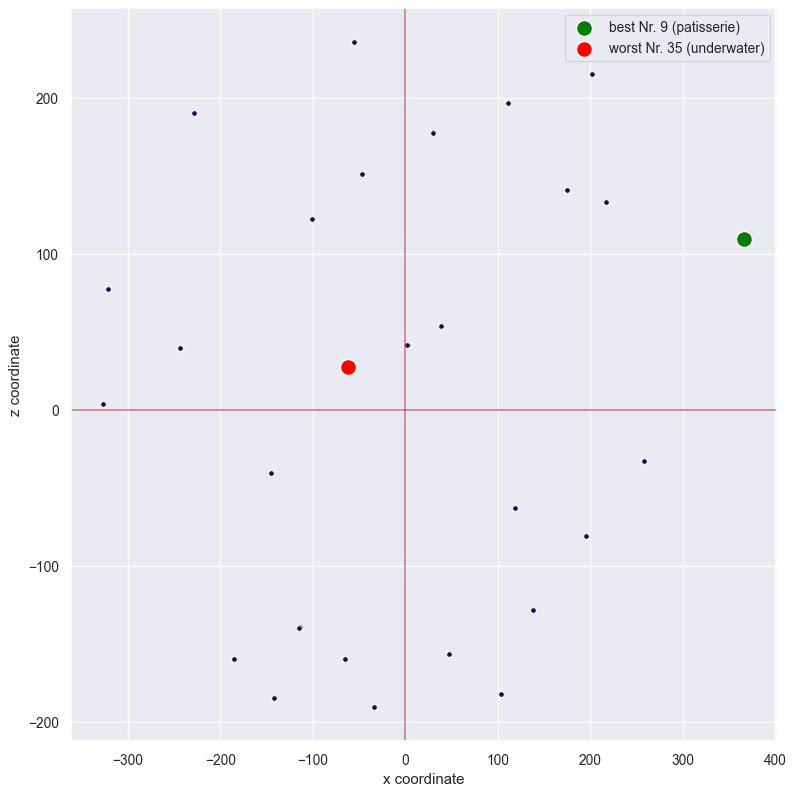
\includegraphics[width=100mm]{figures/best_worst_starting_locations.png}
	\caption[Locations of best and worst starting locations in city]{the locations of the best and worst starting locations inside the city coordinates.}
	\label{fig:best_worst_locs}
\end{figure}


\subsection{Reaction times}

For finding the fastest and the slowest performance among the 28 starting locations, the medians of reaction times grouped by the starting locations were Calculated.\\
The starting location number 51 which was a wine shop, hence a context meaningful location, with the median of 4.63s and the difference of 1.38s from the overall median (6.01) was the fastest location. See figure \ref{fig:fastest_loc}.\\

\begin{figure}[h!]
	\centering
	\begin{subfigure}[b]{0.48\linewidth}
		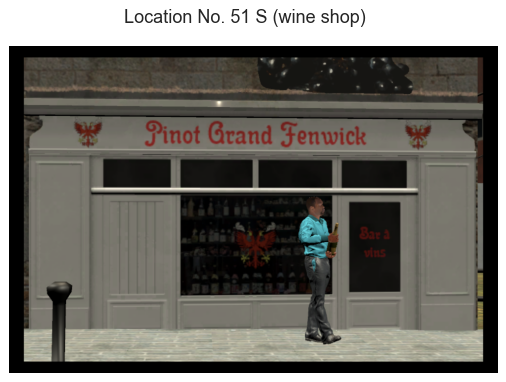
\includegraphics[width=\linewidth]{figures/fastest_loc_RT_withHA_23.png}
		\caption{fastest starting location}
		\label{fig:fastest_loc}
	\end{subfigure}
	\begin{subfigure}[b]{0.48\linewidth}
		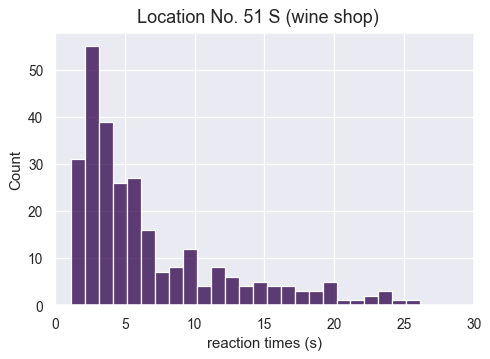
\includegraphics[width=\linewidth]{figures/fastest_loc_RT_dist_51_23.png}
		\caption{reaction times at location 51 (\%)}
		\label{fig:fastest_loc_dist}
	\end{subfigure}
	
	\caption[Fastest starting location]{the fastest starting location is chosen by taking the least median reaction time among all starting locations.}
\end{figure}
\label{fig:fastest_location}


Furthermore, the starting location 35, the residential not context meaningful location with the worst angular deviation performance with the median of 7.75s and overall distance of 1.74s from the overall median (6.01) was the slowest location among the 28. See figure \ref{fig:slowest_loc}.

\begin{figure}[!h]
	\begin{subfigure}[b]{0.48\linewidth}
		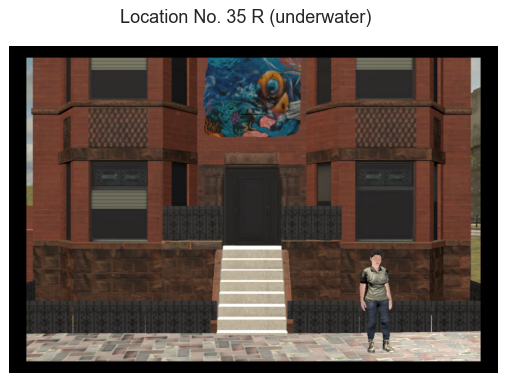
\includegraphics[width=\linewidth]{figures/worst_loc_angular_error__withHA_23.png}
		\caption{slowest starting location}
		\label{fig:slowest_loc}
	\end{subfigure}
	\begin{subfigure}[b]{0.48\linewidth}
		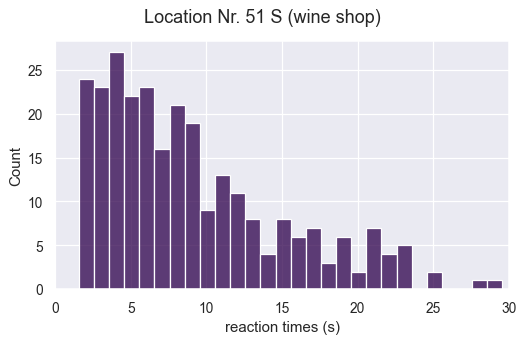
\includegraphics[width=\linewidth]{figures/slowest_loc_RT_dist_35_23.png}
		\caption{distribution of reaction times at location 35 (\%)}
		\label{fig:best_angular_dist_35}
	\end{subfigure}
	
	\caption[Slowest starting location]{the slowest starting location is chosen by taking the highest median of reaction times among all starting locations.}
\end{figure}
\label{fig:slowest_location}

\begin{figure}[h]
	\centering
	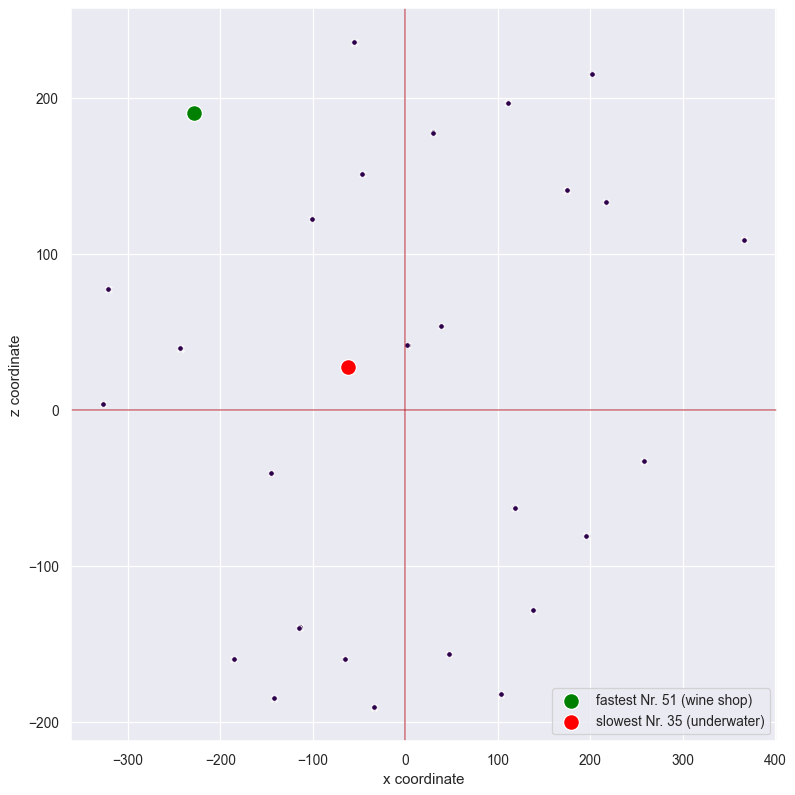
\includegraphics[width=100mm]{figures/fastest_slowest_starting_locations_RT.png}
	\caption[Locations of fastest and slowest starting locations in city]{the locations of the fastest and the slowest starting locations inside the city coordinates.}
	\label{fig:fastest_slowest_locs}
\end{figure}

\section{Linear mixed effects model (absolute angular error)}

\subsection{Absolute angular deviation}

\subsection{Reaction times}

\todo{
	- analysis results to be added
}